\documentclass[letterpaper,9pt,twocolumn,twoside,]{pinp}

%% Some pieces required from the pandoc template
\providecommand{\tightlist}{%
  \setlength{\itemsep}{0pt}\setlength{\parskip}{0pt}}

% Use the lineno option to display guide line numbers if required.
% Note that the use of elements such as single-column equations
% may affect the guide line number alignment.

\usepackage[T1]{fontenc}
\usepackage[utf8]{inputenc}

% pinp change: the geometry package layout settings need to be set here, not in pinp.cls
\geometry{layoutsize={0.95588\paperwidth,0.98864\paperheight},%
  layouthoffset=0.02206\paperwidth, layoutvoffset=0.00568\paperheight}

\definecolor{pinpblue}{HTML}{185FAF}  % imagecolorpicker on blue for new R logo
\definecolor{pnasbluetext}{RGB}{101,0,0} %


\microtypesetup{disable}
\usepackage{booktabs}
\usepackage{longtable}
\usepackage{array}
\usepackage{multirow}
\usepackage{wrapfig}
\usepackage{float}
\usepackage{colortbl}
\usepackage{pdflscape}
\usepackage{tabu}
\usepackage{threeparttable}
\usepackage{threeparttablex}
\usepackage[normalem]{ulem}
\usepackage{makecell}
\usepackage{xcolor}

\title{Predicting Student Performance from Background and Traits}

\author[]{520102934, 530674313, 530341851, 530209908, 520009998}


\setcounter{secnumdepth}{0}

% Please give the surname of the lead author for the running footer
\leadauthor{}

% Keywords are not mandatory, but authors are strongly encouraged to provide them. If provided, please include two to five keywords, separated by the pipe symbol, e.g:
 

\begin{abstract}
The aim of this study is to predict students' final grades by analyzing
their socio-demographic characteristics, academic background, and other
traits. Utilizing two data sets from Portuguese secondary schools, we
applied multiple linear regression, backward selection, and stepwise
model selection to identify key factors that impact final grades in Math
and Portuguese subjects. The results indicate that previous grades, such
as G1 and G2, play a significant role in predicting final performance,
alongside factors like family relationships, commute time, and parental
education. By identifying these predictive factors, we aim to support
educators and policymakers in improving academic outcomes and guiding
targeted interventions for student success.
\end{abstract}

\dates{This version was compiled on \today} 


% initially we use doi so keep for backwards compatibility
% new name is doi_footer

\pinpfootercontents{L02G06}

\begin{document}

% Optional adjustment to line up main text (after abstract) of first page with line numbers, when using both lineno and twocolumn options.
% You should only change this length when you've finalised the article contents.
\verticaladjustment{-2pt}

\maketitle
\thispagestyle{firststyle}
\ifthenelse{\boolean{shortarticle}}{\ifthenelse{\boolean{singlecolumn}}{\abscontentformatted}{\abscontent}}{}

% If your first paragraph (i.e. with the \dropcap) contains a list environment (quote, quotation, theorem, definition, enumerate, itemize...), the line after the list may have some extra indentation. If this is the case, add \parshape=0 to the end of the list environment.


\subsection{Introduction}\label{introduction}

Education is essential to the economic growth of all countries. It is
important for humans to receive primary education and secondary
education both for improving society and themselves (Hanushek \&
WoBmann, 2010). Governments also have programs to support low income
families financially so the children can get early education. One of the
studies conducted for finding correlation between students'
socio-demographic background and academic performances has found that
students from deprived areas perform not as well as their counterparts
(Thiele, Singleton, Pope, \& Stanistreet, 2014). In this paper, we are
using two data sets from two schools in Portugal to determine whether we
can predict student grades via their background and traits.

While it is integral to predict a student's final grade, we are more
interested in the factors that influence students grades and how to
influence those factors to help improve students' performances on the
final grade. This will help our target audience of educators and
students alike for what they could work on to improve grades in general.
We aim to predict students' final grades accurately using multiple
linear regression and interpret the equation to find which qualities of
students impact how much of their final grades.

\subsection{Dataset Description}\label{dataset-description}

The student performance is from two Portuguese secondary schools and
includes student grades, demographic, social and school related features
collected from school reports and surveys. The student performance data
set is divided into two subjects, Math and Portuguese. Both data sets
have 32 features and a predictive variable G3, the final grade students
get for the subject. G1 and G2 are first and second period grades and
are also strongly correlated with G3. There are no missing values.

In both data sets, there are 9 binary types, 8 nominal categorical data
types, 5 ordinal categorical data types, 6 likert scale data types, and
5 discrete numerical data types of columns in the data sets. {[}See
Appendix{]} G3 is a score between 0 to 20. We chose to remove rows where
G3 is 0 because they are outliers and students might be absent on the
final test day in which the scenario doesn't represent how we can help
students get better grades. We also found that there is an outlier in
the Portuguese data set where G3 is 1 so we removed that student. After
filtering, the Math data set has 357 students and the Portuguese data
set has 648 students. Figure 1 shows the distribution of the predictive
variable G3 for both data sets before filtering 0 and 1. (see in
Appendix)

\subsection{Analysis}\label{analysis}

\subsubsection{Model selection}\label{model-selection}

For the Model selection part, we remove the data we don't want to
include through \texttt{filter(G3!=0)} and scale() function; We also use
helper functions like \texttt{calculate\_rmse}, \texttt{calculate\_r2},
and \texttt{calculate\_adj\_r2} for better calculations and finding key
predictor. The result table are shown below:

\begin{table}[!h]
\centering
\caption{\label{tab:model selection}Model Performance Results for Portuguese and Math Datasets}
\centering
\resizebox{\ifdim\width>\linewidth\linewidth\else\width\fi}{!}{
\begin{tabular}[t]{llrrrrrr}
\toprule
Model & Dataset & RMSE\_Train & R2\_Train & Adj\_R2\_Train & Adj\_R2\_Test & RMSE\_Test & R2\_Test\\
\midrule
Refined Linear Model & Portguese & 0.8363 & 0.9014 & 0.8988 & 0.8941 & 0.8324 & 0.9003\\
Refined Log-Transformed Model & Portguese & 10.0314 & -13.1919 & -13.5880 & -14.5016 & 10.0434 & -13.5174\\
Backward Model & Portguese & 0.8208 & 0.9050 & 0.9016 & 0.8872 & 0.8493 & 0.8962\\
Stepwise Model & Portguese & 0.8208 & 0.9050 & 0.9016 & 0.8872 & 0.8493 & 0.8962\\
Refined Linear Model & Math & 0.7847 & 0.9381 & 0.9368 & 0.9282 & 0.8604 & 0.9315\\
\addlinespace
Refined Log-Transformed Model & Math & 9.8094 & -8.6716 & -9.2066 & -7.6057 & 9.0400 & -6.5602\\
Backward Model & Math & 0.7814 & 0.9386 & 0.9374 & 0.9283 & 0.8595 & 0.9317\\
Stepwise Model & Math & 0.7774 & 0.9393 & 0.9377 & 0.9289 & 0.8520 & 0.9328\\
\bottomrule
\end{tabular}}
\end{table}

Based on RMSE and R² values, the backward model is most appropriate for
the Portguese set, the reasons are: 1.Superior Performance: Slightly
better RMSE and R² values compared to the Refined Linear Model (0.8208
vs 0.8362 in RMSE train, 0.9049 vs 0.9013 in R² train).
2.Generalization: Similar performance metrics on training and testing
sets suggest the model generalizes well to unseen data. And the stepwise
model is most appropriate for Math set, the reasons are: 1.it has the
lowest RMSE in train (0.7774) and test (0.8520), high R² value of
(0.9393 in train and 0.9328 in test) and high adjusted R² values, 2..

\subsubsection{Assumption checks (plots see in
Appendix)}\label{assumption-checks-plots-see-in-appendix}

To assess the linearity assumption, visual inspection of the residuals
vs.~fitted values plots was conducted. Ideally, residuals should be
randomly distributed around zero, indicating linearity. For both the
Math and Portuguese datasets, scatter plots with linear regression lines
between G3 and each predictor variable were examined. If the smoother
(red line) in the residual plots remains near zero without a discernible
pattern, the linearity assumption can be considered reasonably
satisfied. The homoscedasticity assumption requires that the variance of
residuals remains constant across all fitted values, meaning that
residuals should be evenly distributed around the zero line without
patterns of increasing or decreasing spread. In a residual vs.~fitted
values plot, a constant spread of residuals suggests that
homoscedasticity is likely satisfied, whereas a funnel or fan shape,
where variance increases or decreases with fitted values, would indicate
heteroscedasticity. The assumption of normality of residuals is assessed
using Q-Q plots for both models, where residuals should ideally fall
along a 45-degree reference line, indicating a normal distribution.
Deviations from this line, especially at the tails, suggest potential
departures from normality; while minor deviations are generally
acceptable, larger deviations, such as heavy tails, may impact the
validity of the model assumptions. The independence of residuals
assumption implies that residuals are uncorrelated with one another,
which is essential to ensure the validity of the model's inferences.
While detecting such independence visually can be challenging,
particularly in time-series or spatial data where patterns or clusters
may indicate dependency, it is generally assumed in cases without time
or spatial ordering, unless there are known violations in the data
collection process. When all assumptions, including independence, are
reasonably satisfied, the model fit is considered adequate and reliable
for inference.

\subsection{Results}\label{results}

For the Portuguese data set, based on RMSE and R² values, the backward
linear model is the most suitable, and the key factors filtered by the
backward selection process are as follows. G2 (second semester grade) :
has the greatest impact on final grade, with a normalization coefficient
of 0.76, indicating a positive effect. G1 (first semester grade) : The
normalization coefficient is 0.18, which has a strong positive effect on
the final grade. traveltime (commute time) and Medu (mother's education
level) also had a positive impact on the target variable, with
standardization coefficients of 0.16 and 0.11, respectively. age has a
positive effect on the score, but the effect is small, and the
standardization coefficient is 0.09. Fjobhealth (maternal employment as
a health field) has the strongest negative effect on performance, with a
normalization coefficient of -0.72. Fjobteacher, Fjobother and
Fjobservices also have negative effects, with coefficients of -0.43,
-0.41 and -0.33, respectively. Variables such as sexM (gender being
male), failures (number of school failures), and schoolMS (type of
school being MS) also had negative effects, with values of -0.24, -0.18,
and -0.16, respectively. absences (number of absences) had very little
effect on the target variable, with a normalization coefficient close to
0. Through this study, we can note that the influence of previous grades
(G1 and G2) on students' G3 grades is very large. For lower grade
students, higher final grades (G3) can be obtained by improving their
grades in the first and second terms. The number of academic failures
has a negative impact on the score, and the coefficient is -0.18.
Students can avoid the failure in the subject examination as much as
possible, and improve the final score through reasonable study plan,
time management and effective study methods. Having parents in certain
occupations (e.g., health, teaching, other occupations, services) has a
negative effect on achievement, especially in the health field
(coefficient -0.72).

For the mathematics data set, the stepwise linear model is the most
suitable, the key factors selected by stepwise are as follows. G2
(second semester grade) is the positive variable that has the greatest
influence on the final grade (G3), and the normalization coefficient is
0.88, indicating that G2 has a great influence on G3. In other words,
improving the grade in the second semester has the biggest boost to the
final grade of math students. famrel (Family Relationship Quality) : The
standardization coefficient is 0.14. This shows that students with
better family relationships usually perform better, and family support
plays a positive role in students' learning. The G1 (first semester
grade) normalization coefficient of 0.10 also has a positive effect on
G3, indicating that the first semester grade is still an important
factor in the final grade, but its effect is much smaller than that of
G2. The health standardization coefficient is 0.06, which has a small
positive effect on G3, and students' health status has some effect on
their final grades. In general, for math students, as well as Portuguese
students, previous academic records also play a crucial role in the
final score of G3, especially G2, and family relationships and
maintaining good health also play a role in the final score of students.

\subsection{Discussion and conclusion}\label{discussion-and-conclusion}

Our analysis highlights several important findings regarding factors
influencing students' academic performance in Math and Portuguese. Key
determinants include prior academic grades (G1 and G2), which were
strong predictors of final grades (G3), and socio-demographic factors
like family support, commute time, and parental occupation. For example,
G2 (second term grade) showed a particularly high influence on G3,
suggesting that students' performance improves if they achieve
consistently throughout the year. Furthermore, factors such as family
relationships and student health demonstrated positive impacts,
indicating the broader role of supportive environments on academic
achievement.

This study has a few limitations that may impact the generalizability of
our findings. Firstly, the reliance on linear regression and stepwise
selection may simplify the complex, potentially non-linear relationships
among predictors. Additionally, while prior grades and demographic
factors were well-represented, some influential variables like students'
self-motivation and study habits were not included, limiting the depth
of our insights.

To address these limitations, future research could explore more
sophisticated, non-linear models such as random forests or decision
trees, which capture complex relationships between variables more
effectively. Moreover, gathering time-series data could provide insights
into how student performance evolves over time, enabling more
personalized predictive models. Examining interactions between factors
(e.g., study time and social activities) could also produce a deeper
understanding of how combined influences impact academic success.

The findings from this study provide insights for applications in
educational settings. For instance, early identification of at-risk
students could be achieved by monitoring G1 and G2 scores, allowing
schools to offer timely interventions. Additionally, promoting family
engagement and addressing health and well-being could further improve
students' academic outcomes. By focusing on these predictive factors,
schools can help create supportive environments that foster student
growth and ultimately contribute to academic success.

Through the regression analysis of the data sets of Portuguese and
mathematics, we can draw the following conclusion: Among the factors
affecting students' final grades (G3), the previous grades (G1 and G2)
play a crucial role, especially the second semester grades (G2) have the
greatest impact on the final grades. For Portuguese students, G2 and G1
have significant positive effects, and family factors such as mother's
occupation and education level also have certain effects. For math
students, good family relationships and health had a positive impact on
achievement. Overall, improving early grades and maintaining good family
relationships and health play an important role in improving students'
final grades.

\clearpage

\subsection{Appendix}\label{appendix}

Figure 1

\begin{center}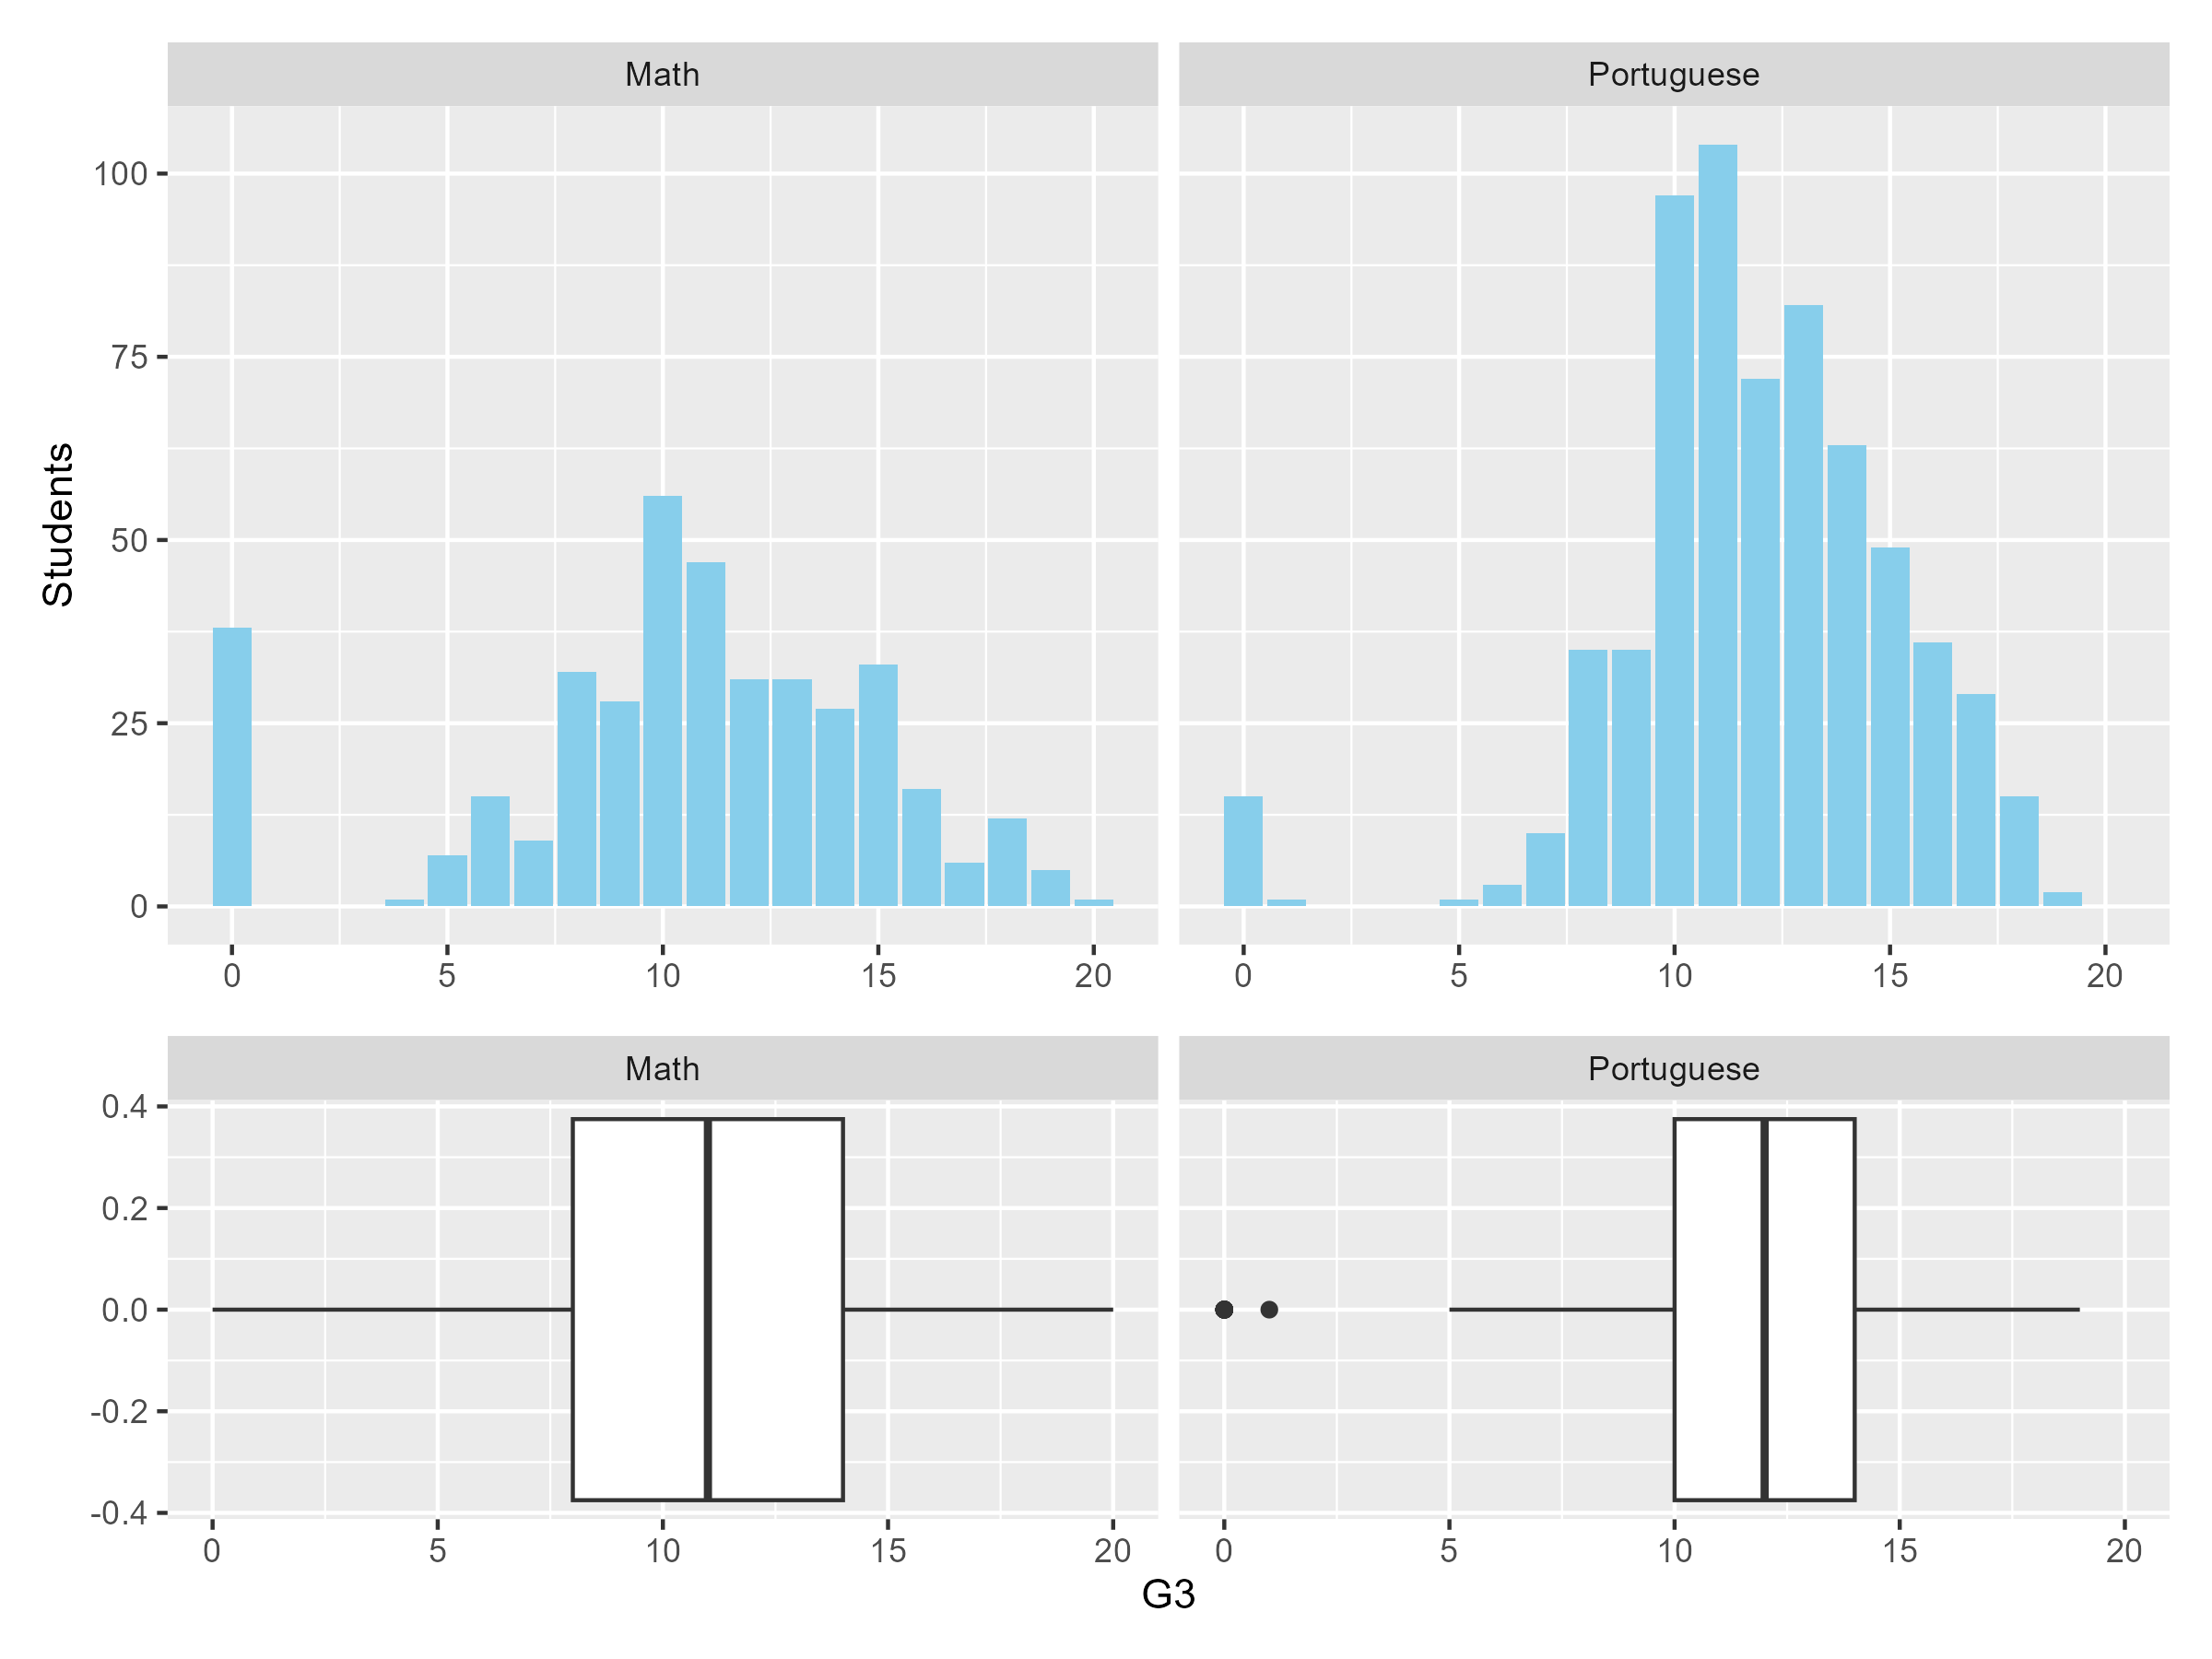
\includegraphics[width=1\linewidth]{combined_plot} \end{center}

Table of summary of different type of features in both Math and
Portuguese Dataset

\begin{center}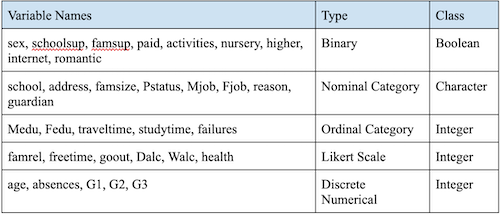
\includegraphics[width=1\linewidth]{table_img} 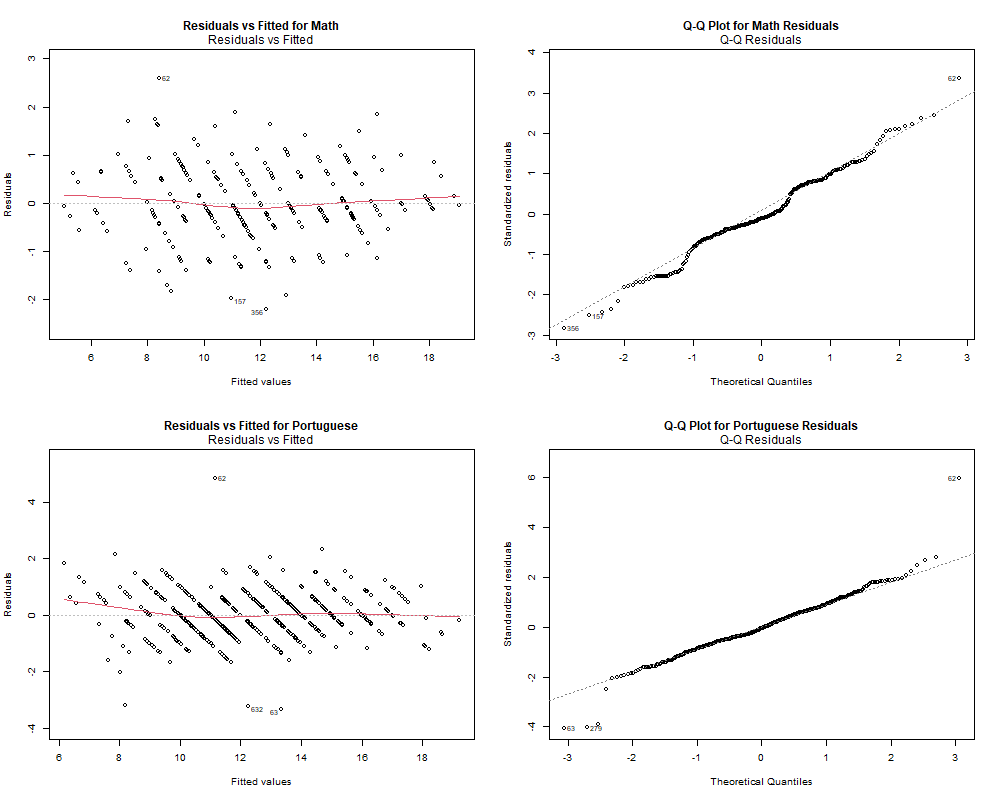
\includegraphics[width=1\linewidth]{combined_diagnostics} \end{center}

\newpage

\subsection{References}\label{references}

\begin{itemize}
\item
  Cortez, P. (2014). Student Performance. Retrieved from
  \url{https://archive.ics.uci.edu/dataset/320/student+performance}.
\item
  Eddelbuettel, D. \& Balamuta, J. (2017). pinp: Pinp is not PNAS. R
  package version
  0.0.2,\url{https://cran.r-project.org/web/packages/pinp/readme/README.html}.
\item
  Hanushek, E., \& WoBmann, L. (2010). Education and Economic Growth.
  Economics of Education, 1(1), 63. Retrieved from
  \url{https://www.google.com.au/books/edition/The_Economics_of_Education/s-jEkQEACAAJ?hl=en}.
\item
  Pedersen T (2024). patchwork: The Composer of Plots. R package version
  1.3.0.9000,
  \href{https://github.com/thomasp85/patchwork,\%20https://patchwork.data-imaginist.com}{https://github.com/thomasp85/patchwork,
  https://patchwork.data-imaginist.com}.
\item
  Thiele, T., Singleton, A., Pope, D., \& Stanistreet, D. (2014).
  Predicting students' academic performance based on school and
  socio-demographic characteristics. Studies in Higher Education, 41(8),
  1424--1446.\url{https://doi.org/10.1080/03075079.2014.974528}.
\item
  Wickham H (2016). ggplot2: Elegant Graphics for Data Analysis.
  Springer-Verlag New York. ISBN 978-3-319-24277-4,
  \url{https://ggplot2.tidyverse.org}.
\item
  Wickham H, François R, Henry L, Müller K, Vaughan D (2023). dplyr: A
  Grammar of Data Manipulation. R package version 1.1.4,
  \url{https://dplyr.tidyverse.org}.
\end{itemize}

%\showmatmethods

\pnasbreak 

\bibliography{pinp}
\bibliographystyle{jss}



\end{document}
